\documentclass{report} 
\title{Appendix 3}
\date{Started 5 Nov 2024}
\author{Malcolm}
\usepackage{amsmath} %import math
\usepackage{mathtools} %more math
\usepackage{amssymb} %for QED symbol
\usepackage{amsthm} %
\usepackage{bm}%bold math
\usepackage{graphicx} %import imaging
\graphicspath{{./images/}} %set imaging path
\begin{document}
\maketitle

\tableofcontents

\appendix
\chapter{Probability}

\section{Fundamental concepts}

\subsection{Permutations and Combinations, Binomial Coefficient}
\textbf{$k$-permutations}\\
Starting with $n$ distinct objects, and letting $k$ be some positive integer where $k\leq n$, 
consider counting the number of different ways that we ca  pick $k$ out of these $n$ objects and arrange them
into a sequence---the number of distinct $k$-object sequences.\\
\vspace{1mm}\\
We first have $n$ choices for the first object. 
Having chosen the first, there are only $n-1$ possible choices for the second, $n-2$ for the third, and so on.
This continues until we have chosen $k-1$ objects, leaving us with $n-(k-1)$ choices for the last one. The 
number of possible sequences, called \textit{$k$-permutations}, can be written as
\begin{equation*}
n(n-1)\cdots(n-k+1)
\end{equation*}
This can be rewritten, giving us
\begin{align*}
n(n-1)\cdots(n-k+1)&=\frac{n(n-1)\cdots(n-k+1)(n-k)\cdots2\cdot1}{(n-k)\cdots2\cdot1}\\
&=\frac{n!}{(n-k)!}
\end{align*}
See that in the special case where $k=n$ we have
\begin{equation*}
n(n-1)(n-2)\cdots2\cdot1=n!
\end{equation*}
(This can also be seen from substituting $k=n$ into the formula and recalling the convention $0!=1$.)\\
(next page)
\newpage
\noindent\textbf{Reordering a set}\\
Starting with $k$ objects, consider trying to find how many ways can we order them in a set of $k$ elements. 
This follows a fairly similar principle to permutation; think of having $k$ `slots' to order $k$ elements in: 
the first `slot' has $k$ possible inputs, the second $k-1$ and so on. See that this just gives us $k!$.\\
\vspace{1mm}\\
\textbf{Combinations}\\
Combinations can be viewed as counting the number of $k$-element subsets of a given $n$-element set.
Combinations are different from permutations in that
\textit{there is no ordering of selected elements}. For instance, where the 2-permutations of the letters 
A, B, C, and D are
\begin{equation*}
\text{AB, BA, AC, CA, AD, DA, BC, CB, BD, DB, CD, DC}
\end{equation*}
the \textit{combinations} of two out of these four letters are
\begin{equation*}
\text{AB, AC, AD, BC, BD, CD}
\end{equation*}
See that the `duplicates' are grouped together; for instance AB and BA are not viewed as distinct.\\
\vspace{1mm}\\
This reasoning can be generalised: each combination is associated with $k!$ `duplicate' $k$-permutations---all
`duplicate' permutations of any given combination is just
that permutation reordered for the maximum number of times:
\begin{equation*}
\text{(any single combination of length $k$)}\cdot k!=\text{(permutations of that combination)}
\end{equation*}
The number $n!/(n-k)!$ of $k$-permutations is equal to the number of combinations times $k!$. Hence the number of
possible combinations is equal to
\begin{equation*}
\frac{n!}{k!\,(n-k)!}
\end{equation*}
\textbf{Binomial Coefficient}\\
Consider a bernoulli process with probability $p$. We want the probility of $k$ `successes' in $n$ trials. 
See that the probability of one \textit{specific} sequence of $n$ trials yielding $k$ `successes' would be
\begin{equation*}
p^k(1-p)^{n-k}
\end{equation*}
We obtain the desired probability by multiplying this by the number of \textit{combinations} of $k$ `successes' we
can obtain in $n$ trials: 
\begin{equation*}
\binom{n}{k}p^k(1-p)^{n-k}
\end{equation*}
(think tossing a coin three times and obtaining two heads---the heads might occur on 
the first and third tosses, or other \textit{combinations} of trials).
\newpage

\subsection{Expectation and Variance}
\textbf{Expectation}\\
We define the \textit{expected value} of a random variable $X$ with a PMF $p_X$ by
\begin{equation*}
\boxed{\mathbb{E}[X]=\sum_xxp_X(x)}
\end{equation*}
\textbf{Variance and Standard Deviation}\\
We define the \textit{variance} associated with a random variable $X$ as
\begin{equation*}
\boxed{\text{var}(X)=\mathbb{E}\left[(X-\mathbb{E}[X])^2\right]=\sum_x(X-\mathbb{E}[X])^2p_X(x)}
\end{equation*}
(See that the because of the square the variance is always nonnegative). The variance provides a measure of
dispersion of $X$ around the mean. Another measure of dispersion is the \textit{Standard deviation} of $X$, which 
is defined as the square root of the variance and is denoted by $\sigma_X$:
\begin{equation*}
\boxed{\sigma_X=\sqrt{\text{var}(X)}}
\end{equation*}
The standard deviation is often easier to interpret because it has the same units as $X$.
\newpage

\subsection{Expected value of a function of a RV}
\textbf{Expectation of a function}\\
Let $X$ be a RV with PMF $p_X$, and let $g(X)$ be a function of $X$. Then the expected value
of the random variable $g(X)$ is given by
\begin{equation*}
\boxed{\mathbb{E}[g(X)]=\sum_xg(x)p_X(x)}
\end{equation*}
This can be shown, since
\begin{equation*}
p_Y(y)=\sum_{\{x|g(x)=y\}}p_X(x)
\end{equation*}
we have
\begin{align*}
\mathbb{E}[g(X)]&=\mathbb{E}[Y]\\
&=\sum_yyp_Y(y)\\
&=\sum_yy\sum_{\{x|g(x)=y\}}p_X(x)\\
&=\sum_y\sum_{\{x|g(x)=y\}}yp_X(x)\\
&=\sum_y\sum_{\{x|g(x)=y\}}g(x)p_X(x)\\
&=\sum_xg(x)p_X(x)
\end{align*}
\textbf{Variance}\\
Using this we can write the variance of $X$ as
\begin{equation*}
\text{var}(X)=\mathbb{E}\left[(X-\mathbb{E}[X])^2\right]
=\sum_x(X-\mathbb{E}[X])^2p_X(x)
\end{equation*}
\newpage

\subsection{Expectation and variance of linear functions}
We show for a random variable $X$, and letting $Y=aX+b$:
\begin{equation*}
\boxed{\mathbb{E}[Y]=a\mathbb{E}[X]+b,\quad
\text{var}(Y)=a^2\text{var}(X)}
\end{equation*}
Linearity of Expectations:
\begin{equation*}
\mathbb{E}[Y]=\sum_x(ax+b)p_X(x)=a\underbrace{\sum_xxp_x(x)}_{=\mathbb{E}[X]}+b\underbrace{\sum_xp_x(x)}_{=1}
=a\mathbb{E}[X]+b
\end{equation*}
Variance:
\begin{align*}
\text{var}(Y)&=\sum_x(ax+b-\mathbb{E}[aX+b])^2p_X(x)\\
&=\sum_x(ax+b-a\mathbb{E}[X]+b)^2p_X(x)\\
&=a^2\sum_x(x-\mathbb{E}[X])^2p_X(x)\\
&=a^2\text{var}(X)
\end{align*}
Note that unless $g(X)$ is a linear function, it is not generally true that $\mathbb{E}[g(X)]$ is equal to 
$g(\mathbb{E}[X])$.

\subsection{Variance in terms of Moments Expression}
We show
\begin{equation*}
\boxed{\text{var}(X)=\mathbb{E}[X^2]-(\mathbb{E}[X])^2}
\end{equation*}
see that
\begin{align*}
\text{var}(X)&=\sum_x(x-\mathbb{E}[X])^2p_X(x)\\
&=\sum_x(x^2-2x\mathbb{E}[X]+(\mathbb{E}[X])^2)p_X(x)\\
&=\sum_xx^2p_X(x)-2\mathbb{E}[X]\sum_xxp_X(x)+(\mathbb{E}[X])^2\sum_xp_X(x)\\
&=\mathbb{E}[X^2]-2(\mathbb{E}[X])^2+(\mathbb{E}[X])^2\\
&=\mathbb{E}[X^2]-(\mathbb{E}[X])^2
\end{align*}
\newpage

\subsection{Expectation and Variance of Bernoulli}
Consider a Bernoulli RV $X$ with PMF
\begin{equation*}
p_X(k)=\begin{cases}
p,&\text{if }k=1.\\
1-p,&\text{if }k=0.
\end{cases}
\end{equation*}
The mean, second moment, and variance of $X$ are as follows:
\begin{align*}
\mathbb{E}[X]&=1\cdot p+0\cdot(1-p)=p\\
\mathbb{E}[X^2]&=1^2\cdot p+0\cdot(1-p)=p\\
\text{var}(X)&=\mathbb{E}[X^2]-(\mathbb{E}[X])^2
=p-p^2=p(1-p)
\end{align*}

\subsection{Expectation of Discrete Uniform}
Consider a Discrete Uniform RV $X$ with PMF, for $k\in[a,b]$:
\begin{equation*}
p_X(k)=\begin{cases}
\frac{1}{b-a+1},&\text{if }k=a,a+1\ldots,b\\
0,&\text{otherwise}.
\end{cases}
\end{equation*}
An illustration is useful here:
\begin{figure}[h]
\begin{center}
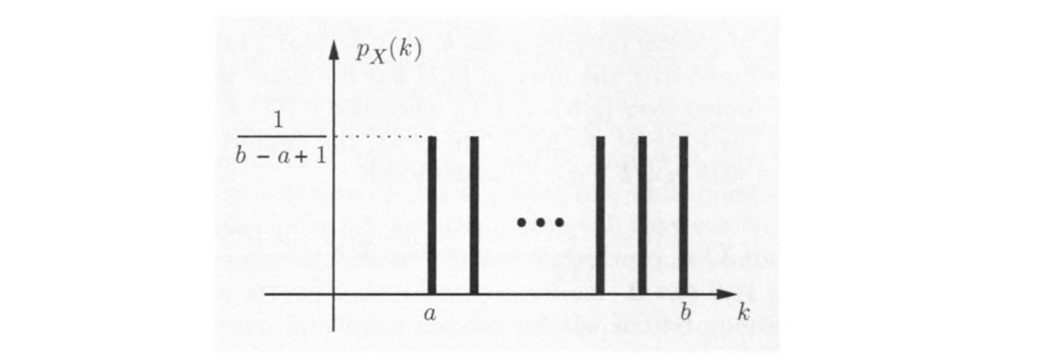
\includegraphics[width=10cm]{1}\\
\end{center}
\textbf{Expectation}\\
Upon inspection one might suppose that the expectation is
\begin{equation*}
\mathbb{E}[X]=\frac{a+b}{2}
\end{equation*}
\end{figure}\\
(next page)
\newpage
\noindent\textbf{Expectation (cont.)}\\
The formula can be elucidated from the definition of the expectation. First see that a sequence
$\sum^b_{k=a}k$ can be written as
\begin{align*}
\sum^b_{k=a}k&=\sum^b_{k=1}k-\sum^{a-1}_{k=1}k\\
&=\frac{(b)(b+1)}{2}-\frac{(a-1)(a)}{2}\quad\text{(see \ref{supnotes:1})}\\
&=\frac{b^2+b-a^2+a}{2}=\frac{(b-a+1)(a+b)}{2}
\end{align*}
The last step isn't easy to factor, but working back from our `hypothesis' for the expectation it coincides.\\
\vspace{1mm}\\
so now we have
\begin{align*}
\mathbb{E}[X]&=\sum^b_{k=a}k\left(\frac{1}{b-a+1}\right)\\
&=\frac{1}{b-a+1}\sum^b_{k=a}k\\
&=\frac{1}{b-a+1}\cdot\frac{(b-a+1)(a+b)}{2}\\
\mathbb{E}[X]&=\frac{(a+b)}{2}
\end{align*}
\newpage

\subsection{Variance of Discrete Uniform}
\textbf{Case for $k\in[1,n]$}:\\
We can obtain the second moment for a discrete uniform distributed over $k\in[1,n]$ as
\begin{align*}
\mathbb{E}[X^2]&=\sum^{n}_{k=1}k^2\left(\frac{1}{n}\right)\\
&=\frac{1}{n}\sum^{n}_{k=1}k^2\\
&=\frac{1}{n}\cdot\frac{n(n+1)(2n+1)}{6}\quad\text{(see \ref{supnotes:4})}\\
&=\frac{(n+1)(2n+1)}{6}
\end{align*}
We then use the formula for variance in terms of moments expression:
\begin{align*}
\text{var}(X)&=\mathbb{E}[X^2]-(\mathbb{E}[X])^2\\
&=\frac{(n+1)(2n+1)}{6}-\left(\frac{n+1}{2}\right)^2\\
&=\frac{1}{12}(n+1)(4n+2-3n-3)\\
&=\frac{n^2-1}{12}
\end{align*}
\textbf{General case} $k\in[a,b]$:\\
For the general case, note that a RV uniformly distributed over an interval $[a,b]$ has the \textit{same variance}
as one which is uniformly distributed over $[1,b-a+1]$---the PMF of the second is just a shifted version
of the PMF of the first.\\
\vspace{1mm}\\
Therefore, the desired variance is given by the first case, but instead with $n=b-a+1$, yielding
\begin{equation*}
\boxed{\text{var}(X)=\frac{(b-a+1)^2-1}{12}=\frac{(b-a)(b-a+2)}{12}}
\end{equation*}
\newpage

\section{Limit Theorems}
\subsection{Sample mean}
\textbf{Definition}\\
Here we discuss asymptomatic behaviour of sequences of random variables. The principal context involves a sequence 
$X_1,X_2,\ldots$ of independent identically distributed random variables with expectation $\mu$ and variance 
$\sigma^2$.
We denote
\begin{equation*}
S_n=X_1+\cdots+X_n
\end{equation*}
to be the sum of the first $n$ of them. Since they are independent we also have
\begin{equation*}
\text{var}(S_n)=\text{var}(X_1)+\ldots+\text{var}(X_n)=n\sigma^2
\end{equation*}
See that the distribution of $S_n$ spreads out (it's variance increases) as $n$ increases and doesn't have a 
meaningful limit. Consider instead the \textit{sample mean}
\begin{equation*}
M_n=\frac{X_1+\cdots+X_n}{n}=\frac{S_n}{n}
\end{equation*}
\textbf{Expectation and Variance}\\
We have the expectation as
\begin{align*}
\mathbb{E}[M_n]&=\frac{\mathbb{E}[X_1+\ldots+X_n]}{n}\\
&=\frac{\mathbb{E}[X_1]+\ldots+\mathbb{E}[X_n]}{n}\\
&=\frac{n\mu}{n}=\mu
\end{align*}
and the variance as
\begin{equation*}
\text{var}(M_n)=\frac{1}{n^2}\,\text{var}(S_n)=\frac{\sigma^2}{n}
\end{equation*}
See that the variance of $M_n$ decreases to 0 as $n$ increases.\\
\vspace{1mm}\\
With this consider a new random variable, that we modify based off $M_n$ and $S_n$:
\begin{equation*}
Z_n=\frac{S_n-n\mu}{\sigma\sqrt{n}}
\end{equation*}
This has the properties
\begin{equation*}
\mathbb{E}[Z_n]=0,\quad\text{var}(Z_n)=\frac{\text{var}(S_n-n\mu)}{\sigma^2n}=1
\end{equation*}
\newpage

\subsection{Markov Inequality}
\textbf{Definition}\\
Here we consider the \textit{Markov inequality}. Loosely speaking it asserts that
if a \textit{nonnegative} random variable has a small mean, then the probability that it takes a large value must
also be small:
\begin{equation*}
\boxed{\mathbb{P}(X\geq a)\leq\frac{\mathbb{E}[X]}{a},\quad\text{if $X\geq0$ and $a>0$.}}
\end{equation*}
(intuitively, as $a$ increases, the probability that $X$ is greater than it decreases)
\begin{figure}[h]
\textbf{Justification}\\
Consider fixing a positive number $a$ and considering the random variable $Y_a$ defined by
\begin{equation*}
Y_a=\begin{cases}
0,&\text{if }X<a,\\
a,&\text{if }X\geq a.
\end{cases}
\end{equation*}
See that the relation 
\begin{equation*}
Y_a\leq X
\end{equation*}
always holds and therefore
\begin{equation*}
\mathbb{E}[Y_a]\leq\mathbb{E}[X]
\end{equation*}
\begin{center}
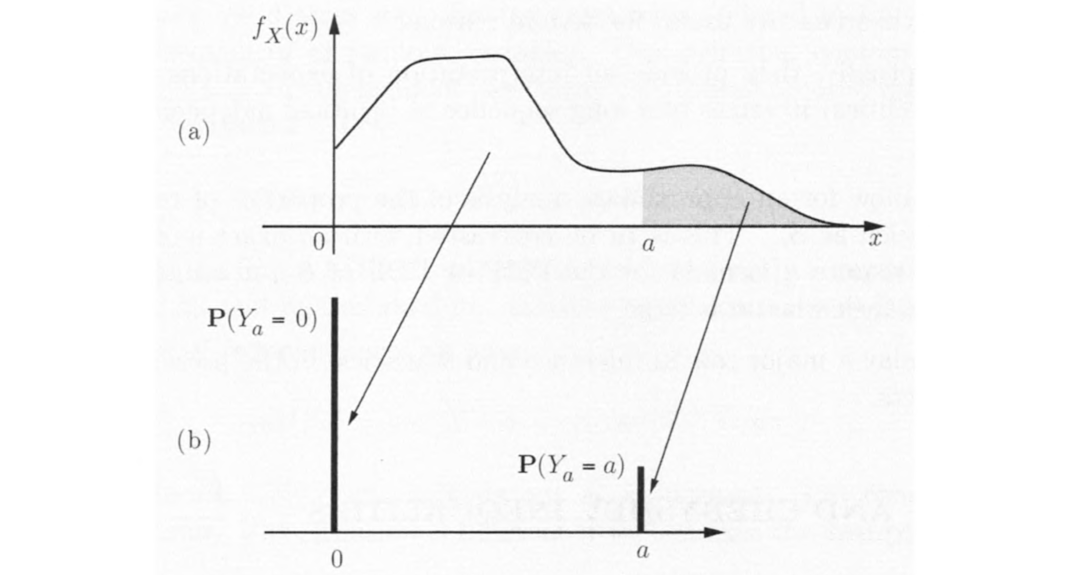
\includegraphics[width=10cm]{2}\\
\end{center}
See that all of the probability mass in the PDF of $X$ between 0 and $a$ is assigned to 0, and that above $a$
assigned to $a$. Since mass is shifted to the left, the expectation can only decrease:
\begin{equation*}
\mathbb{E}[X]\geq\mathbb{E}[Y_a]=a\mathbb{P}(Y_a=a)
=a\mathbb{P}(X\geq a)
\end{equation*}
from which we obtain
\begin{equation*}
a\mathbb{P}(X\geq a)
\leq\mathbb{E}[X]
\end{equation*}
\end{figure}\\
(next page)
\newpage
\noindent\textbf{Another justification}\\
See that if $X\geq0$ and $a>0$:
\begin{align*}
\mathbb{E}[X]=\int^\infty_0&xf_X(x)\,dx\geq\int^\infty_axf_X(x)\,dx\\
&\geq\int^\infty_aaf_X(x)\,dx\\
&=a\mathbb{P}(X\geq a)
\end{align*}
so
\begin{equation*}
\mathbb{E}[X]\geq a\mathbb{P}(X\geq a)
\end{equation*}
and
\begin{equation*}
\mathbb{P}(X\geq a)\leq\frac{\mathbb{E}[X]}{a}
\end{equation*}
\newpage

\subsection{Chebyshev Inequality}
\textbf{Definition}\\
The \textit{Chebyshev inequality}, loosely speaking, asserts that if a random variable has small variance, then
the probability that it takes a value far from its mean is also small: Given a random
variable $X$ with mean $\mu$ and variance $\sigma^2$,
\begin{equation*}
\boxed{\mathbb{P}(|X-\mu|\geq c)\leq\frac{\sigma^2}{c^2},\quad\text{for all $c>0$}}
\end{equation*}
Note that the Chebyshev inequality does not require the random variable to be negative.\\
\vspace{1mm}\\
\textbf{Justification}\\
Consider the nonnegative random variable $(X-\mu)^2$ and apply the Markov inequality with $a=c^2$ to obtain:
\begin{equation*}
\mathbb{P}((X-\mu)^2\geq c^2)\leq\frac{\mathbb{E}\left[(X-\mu)^2\right]}{c^2}=\frac{\sigma^2}{c^2}
\end{equation*}
Now observe that since the event $(X-\mu)^2\geq c^2$ is identical to the event $|X-\mu|\geq c$, so that
\begin{equation*}
\mathbb{P}(|X-\mu|\geq c)=\mathbb{P}((X-\mu)^2\geq c^2)\leq\frac{\sigma^2}{c^2}
\end{equation*}
The Chebyshev inequality tends to be more powerful than the Markov inequality since it also uses information on
the variance of $X$. An alternative form can also be obtained by letting $c=k\sigma, k>0$, which yields
\begin{equation*}
\mathbb{P}(|X-\mu|\geq k\sigma)\leq\frac{\sigma^2}{k^2\sigma^2}=\frac{1}{k^2}
\end{equation*}
(the probability that a random variable takes a value more than $k$ standard deviations away from its mean is at 
most $1/k^2$)\\
\vspace{1mm}\\
\textbf{Another justifcation}\\
For a derivation that doesn't use the Markov inequality, introducing the function
\begin{equation*}
g(x)=\begin{cases}
0,&\text{if }|x-\mu|<c,\\
c^2,&\text{if }|x-\mu|\geq c
\end{cases}
\end{equation*}
since $(x-\mu)^2\geq g(x)$ for all $x$ we can write
\begin{align*}
\sigma^2=\int^\infty_{-\infty}&(x-\mu)^2f_X(x)\,dx\geq
\int^\infty_{-\infty}g(x)f_X(x)\,dx\\
&=c^2\left(\int^{\mu-c}_{-\infty}f_X(x)\,dx+\int_{\mu+c}^\infty f_X(x)\,dx\right)\\
&=c^2\mathbb{P}(|X-\mu|\geq c)
\end{align*}
which can be arranged into the desired inequality.
\newpage

\subsection{}



\newpage

\chapter{Supplementary Notes}

\section{The sum of the first $n$ natural numbers is $n(n+1)/2$}
\label{supnotes:1}
We have that
\begin{equation*}
\sum^i_{i=1}i=1+2+\cdots+n
\end{equation*}
Now consider $2\sum^n_{i=1}i$:
\begin{align*}
2\sum^n_{i=1}i&=2(1+2+\cdots+(n-1)+n)\\
&=(1+2+\cdots+(n-1)+n)+(n+(n-1)+\cdots+2+1)\\
&=(1+n)+(2+(n-1))+\cdots+((n-1)+2)+(n+1)\\
&=(n+1)_1+(n+1)_2+\cdots+(n+1)_n\\
&=n(n+1)
\end{align*}
so
\begin{align*}
2\sum^n_{i=1}i&=n(n+1)\\
\sum^n_{i=1}i&=\frac{n(n+1)}{2}
\end{align*}
\newpage

\section{Telescoping series}
\label{supnotes:2}
Let $\langle b_n\rangle$ be a sequence in $\mathbb{R}$. Let $\langle a_n\rangle$ be a sequence defined as
\begin{equation*}
a_k=b_k-b_{k-1}
\end{equation*}
we show
\begin{equation*}
\boxed{\sum^n_{k=m}a_k=b_n-b_{m-1}}
\end{equation*}
See that
\begin{align*}
\sum^n_{k=m}a_k&=\sum^n_{k=m}(b_k-b_{k-1})\\
&=\sum^n_{k=m}b_k-\sum^n_{k=m}b_{k-1}\\
&=\sum^n_{k=m}b_k-\sum^{n-1}_{k=m-1}b_k\\
&=\left(\sum^{n-1}_{k=m}b_k+b_n\right)-\left(b_{m-1}+\sum^{n-1}_{k=m}b_k\right)\\
&=b_n-b_{m-1}
\end{align*}
\newpage

\section{Sum of series of products of consecutive integers}
\label{supnotes:3}
We show
\begin{align*}
\boxed{\sum^n_{j=1}j(j+1)=1\cdot2+2\cdot3+\cdots
+n(n+1)=\frac{n(n+1)(n+2)}{3}}
\end{align*}
See that
\begin{align*}
3i(i+1)&=i(i+1)(i+2)-i(i+1)(i-1)\\
&=(i+1)((i+1)+1)((i+1)-1)-i(i+1)(i-1)
\end{align*}
Thus we have the basis of a telescoping series (see (\ref{supnotes:2})):
\begin{equation*}
3i(i+1)=b(i+1)-b(i)
\end{equation*}
where
\begin{equation*}
b(i)=i(i+1)(i-1)
\end{equation*}
So we have
\begin{align*}
\sum^n_{j=1}3j(j+1)&=\sum^n_{j=1}(j+1)((j+1)+1)((j+1)-1)-j(j+1)(j-1)\\
&=n(n+1)(n+2)-0(0+1)(0-1)\\
&=n(n+1)(n+2)
\end{align*}
Thus
\begin{equation*}
\sum^n_{j=1}j(j+1)=\frac{n(n+1)(n+2)}{3}
\end{equation*}
\newpage

\section{Sum of sequence of squares}
\label{supnotes:4}
We show
\begin{equation*}
\boxed{\forall n\in\mathbb{N}:
\sum^n_{i=1}i^2=\frac{n(n+1)(2n+1)}{6}}
\end{equation*}
See that this follows from (\ref{supnotes:3}):
\begin{align*}
\sum^n_{i=1}3i(i+1)&=n(n+1)(n+2)\\
\sum^n_{i=1}3i^2+\sum^n_{i=1}3i&=n(n+1)(n+2)\\
\sum^n_{i=1}3i^2&=n(n+1)(n+2)-3\frac{n(n+1)}{2}\quad\text{see (\ref{supnotes:1}))}\\
\sum^n_{i=1}i^2&=\frac{n(n+1)(n+2)}{3}-\frac{n(n+1)}{2}\\
&=\frac{2n(n+1)(n+2)-3n(n+1)}{6}\\
&=\frac{n(n+1)(2n+1)}{6}
\end{align*}














\end{document}
